
\documentclass[preprint,12pt,a4]{standalone}
\usepackage{geometry}   % my added package "geometry"
\geometry{letterpaper,tmargin=1in,bmargin=1in,lmargin=2.5cm,rmargin=2.5cm}
\usepackage{tikz}
\usetikzlibrary{calc,patterns,arrows.meta,shapes.arrows,intersections,positioning}
\usetikzlibrary{decorations.pathmorphing,backgrounds,fit,petri}
\usepackage{standalone}
\begin{document}
	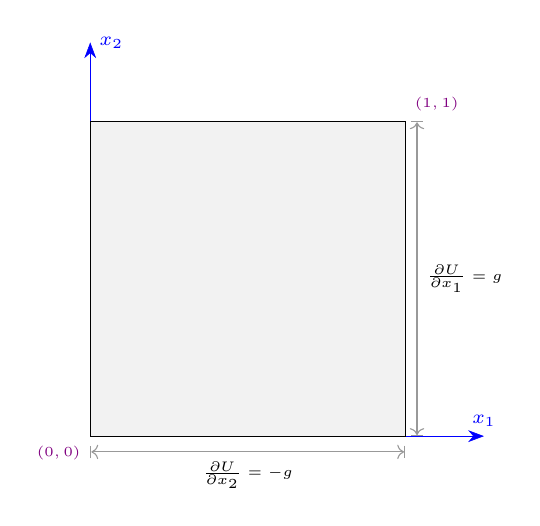
\begin{tikzpicture} [{place/.style={rectangle,draw=blue!50,fill=blue!20,ultra thin,inner sep=0.8mm}},{place2/.style={circle,draw=black!50,ultra thin,inner sep=0.8mm}},{linest/.style={color=gray,ultra thin}}]
	%%coordinates of corners of Beam
	\coordinate (A) at (0.0, 0.0);
	\coordinate (B) at (4.0, 0.0);
	\coordinate (C) at (4.0, 4.0);
	\coordinate (D) at (0.0, 4.0);
	%%axes
	\draw [{Stealth[length=2mm]}-{Stealth[length=2mm]}, help lines,blue] (5,0)node[above,font=\scriptsize]{$x_{1}$} -- (0,0) -- (0,5)node[right,font=\scriptsize] {$x_{2}$};
	%%square
	\draw [fill=gray!10] (A)node[font=\tiny, violet,below left]{$(0,0)$} rectangle  (C)node[font=\tiny, violet,above right]{$(1,1)$};
	
	%\draw [color=black](A)node[font=\tiny, violet,below left]{$(0,0)$} -- (A) -- (B)  -- %(C)node[font=\tiny, violet,above right]{$(1,1)$} -- (D) -- (A);
	%%B.C
	\draw [|<->|,gray!80]($(A)+(0,-0.2)$) --($(B)+(0,-0.2)$) node[fill=white,midway,below, font=\tiny,text=black] {$\frac{\partial{U}}{\partial{x_{2}}} =-g$};
	
	\draw [|<->|,gray!80]($(B)+(0.15,0.0)$)--($(C)+(0.15,0.0)$) node [fill=white,midway, right, font=\tiny, text=black] {$\frac{\partial{U}}{\partial{x_{1}}} =g$};
	\end{tikzpicture}
\end{document}